\chapter{Implementation and Experimental Results}

\section{ParaReal.jl}

Design requirements / goals:
\begin{enumerate}
  \item
    Schedule each stage on a separate process.
  \item
    Prepare the scheduling strategy to be modifiable and extendable.
  \item
    The parareal implementation has to be modular,
    \ie easy to use/adapt for other problems than \ac{LRSIF} formulations of \ac{DRE}.
  \item
    Do not transfer the final solution data back to the calling/managing process.

    For fine resolutions, the storage requirements are immense.
    The overall solution might not fit in memory of one compute node.
    Therefore, it has to be possible that each stage $n$ saves its local solution along $[t_{n-1},t_n]$ directly to disk,
    without sending it to the calling process first.
  \item
    Allow the data transferred be variable in size.

    This is necessary to transmit \ac{LRSIF} of varying rank and therefore storage size depending on $n$ (and $k$).
    However, using Julia's \julia{RemoteChannel} data type, this is trivial.
\end{enumerate}
The result is the \julia{ParaReal.jl} package,
whose properties are described in this section.

The first two requirements are achieved by the abstract type \julia{Schedule},
whose only subtype (for now) is \julia{ProcessesSchedule}.
It takes a list of $N$ worker/process ids, each of which will execute one stage.
Future strategies may be implemented by defining new subtype of \julia{Schedule}, \eg
\julia{ThreadsSchedule} using threads on a single process,
\julia{HybridSchedule} which uses both threads and processes, and
\julia{DaggerSchedule} which uses the abstractions provided by \julia{Dagger.jl}.\footnote{\url{https://github.com/JuliaParallel/Dagger.jl}}

The user interface fulfilling the third requirement is best described using an example:
\lstinputlisting{code/parareal_counting.jl}

This makes it handy to apply the package to problems having different standard nomenclatures,
\eg $U$ as for many parareal papers, or
$X$ as for many matrix \ac{ODE} papers, or
$u$ as for the famous \julia{DifferentialEquations.jl} package~\cite{DifferentialEquations}.

Running the example above yields the following values:
\begin{align*}
  &\julia{Counters(1,0)}, \text{ since} &
  U_1^1 &= F(U_0) \\
  &\julia{Counters(2,0)}, \text{ since} &
  U_2^2 &= F(F(U_0)) \\
  &\julia{Counters(3+2+2,2+4+4)}, \text{ since} &
  U_3^2 &= G(F(F(U_0))) + F(U_2^1) - G(U_2^1) \\
  && U_2^1 &= G(F(U_0)) + F(G(U_0)) - G(G(U_0))
\end{align*}
In the notion of \julia{ParaReal.jl},
$F_n^k$ and $G_n^k$ denote the return values of calls to the fine coarse solvers, respectively,
which may hold more data than just $F(U_n^k)$.
In applications, one is usually interested in the complete trajectory of $U$ on $[t_0,t_f]$.
Therefore, $F_n^k$ usually stores the trajectory on $[t_n,t_{n+1}]$,
of which \julia{ParaReal.value} extracts the (final) value at $t_{n+1}$.
In the example above, both are identical, though.

\todo[inline]{%
  Make code look pretty, maybe put it in the appendix.
  Describe results of code better.
  Note that $U_2^1$ isn't actually computed twice.
  Maybe I should provide a custom update routing to account for this.
}

\subsection{JIT Compilation and Warm-Up}

Julia is a \ac{JIT} compiled language~\cite{Julia},
which means that code is compiled just before it is first executed,
unless it has already been compiled.
Therefore, unless the code has been compiled \ac{AOT},
only the second execution of code is fast.
This effect is called \emph{warm-up}.
As mentioned in~\autoref{sec:pr}, computing the coarse solutions
$G(U_n^*)$ is essentially a sequential operation over all $n$.
The computations of $F(U^*_n)$ can only be parallelized after such a global coarse solve.
Therefore, it is critical that the individual coarse solutions are available as fast as possible.

\todo[inline]{Describe notion of \enquote{ramp-up delay}?}

\begin{figure}[htb]
  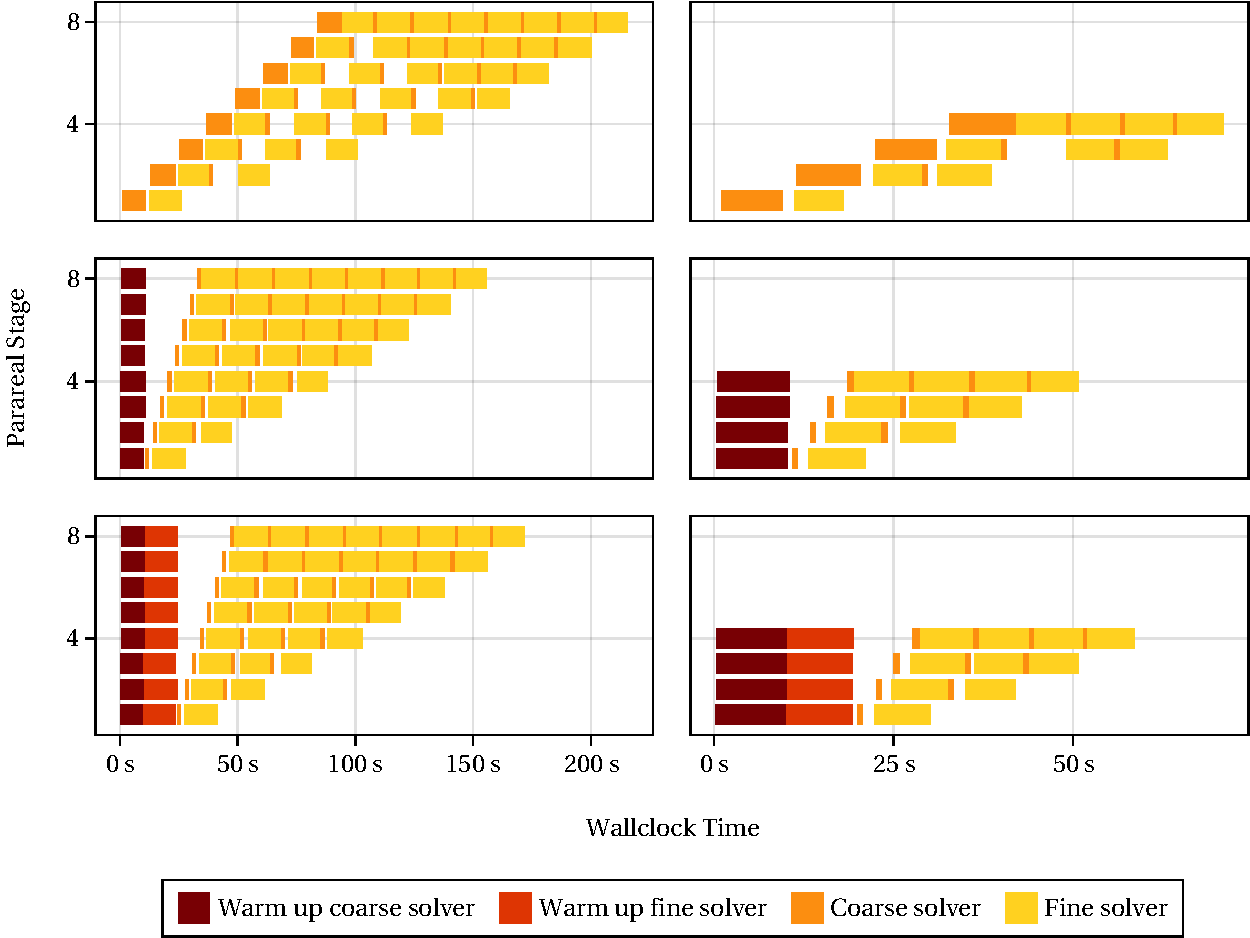
\includegraphics[width=\textwidth]{figures/fig_impl_warmup2.pdf}
  \caption[Timeline diagrams comparing the effect of JIT compiler warm-up.]{%
    Timeline diagrams comparing the effect of \acs{JIT} compiler warm-up.
    Left: 8 processes running on two compute nodes,
    right: 4 processes running on a laptop.
    Top: no warm-up,
    middle: warming up coarse solver \julia{csolve} ($G$),
    bottom warming up coarse and fine solver \julia{fsolve} ($F$).
  }
  \label{fig:impl:warmup}
\end{figure}

\paragraph{Sequential \ac{JIT} compilation}

Without any precautions,
\ac{JIT} compilation of $G$ happens sequentially,
as computing $G(U_n^k)$ is essentially sequential.
This effect is especially severe if the executors of different parareal iterations $(n,k)$ do not share the results of code compilation.
These executors may be processes, threads~(pthreads), or tasks~(green threads).
As of the writing of this thesis,
there is a one-to-one mapping between processes and stages $n$,
which means the compilation happens exactly once per stage $n$ and is reused between refinements $k$.\footnote{%
  As of the writing of this thesis, Julia does not reuse code compiled between processes.
}
This is visible in the first row of \autoref{fig:impl:warmup}
by the first occurrences of $G$ for each stage $n$,
which marks the computation of $G(U_n^0)$,
whose execution time includes compilation time.

\paragraph{Parallel \acs{AOT} compilation}

Since \julia{ParaReal.jl} is independent of $F$ and $G$ as well as the actual data type of the underlying \ac{IVP},
full \ac{AOT} compilation is difficult, and has to be done by users of the package.
A more naive approach is to manually warm up critical parts of the code by executing them before they are actually needed.
In the context of \julia{ParaReal.jl},
doing so allows to perform the compilation in parallel,
which significantly decreases the time to compute all coarse solutions $G(U_n^*)$.
This is visible in the middle and bottom rows of \autoref{fig:impl:warmup}.
$F$ and $G$ have a lot of code in common,\footnote{%
  For example, the Lyapunov solvers will be called with arguments having the exact same types,
  \ie they will call the same method internally.
  Unless that method has been inlined, the results of its compilation will be reused.
}
such that warming up both shows a much smaller improvement compared to just warming up the coarse solver $G$.

\paragraph{Precompilation}

Besides reducing the delay of executing $F$ and $G$,
it is also important to reduce the delay of any code from \julia{ParaReal.jl} that doesn't depend on them.
The package is merely responsible for orchestrating the execution of the parareal iterations $(n,k)$.
Therefore, the delay of the first execution of \julia{ParaReal.jl} code is dominated by type inference.\footnote{%
  At least it likely is. Taking measurements is highly non-trivial and out of the scope of this thesis.
  For more details see: \url{https://julialang.org/blog/2020/08/invalidations/}
}
The time spent on type inference can be minimized by precompilation,
which happens when the package is first loaded,
and whose results are cached and reused when the package is loaded again.
Exploiting this is highly non-trivial and out of the scope of this thesis.\footnote{\url{https://julialang.org/blog/2021/01/precompile_tutorial/}}

\todo[inline]{%
How to cite these webpages properly?
Should I do anything about the speculation in the paragraph, or the exposure of which in the footnote?
}

\todo[inline]{Where should I put the next paragraph?}

Note that if the coarse solver is warmed up,
for $n=1$ the actual solve $G(U_0^0)$ is barely visible,
because it is the exact call used for \ac{JIT} warm-up.
For $n\geq 2$, the execution time of computing $G(U_{n-1}^0)$ is noticeably larger,
which may be due to type inference.
The local problem instance is updated for the new initial value $U_{n-1}^0$,
which might cause some method invalidations.
This gives more room for improvement.

\subsection{Lack of Asynchronous Data Transfer}
\todo[inline]{Should this just be another paragraph?}

A common strategy to improve CPU utilization is to perform data transfers between processes asynchronously.
Julia offers the \julia{RemoteChannel} data structure for this purpose.
As of the writing of this thesis,
the \julia{RemoteChannel} is not thread-safe.\footnote{\url{https://github.com/JuliaLang/julia/issues/37706}}
More specifically, it must be used from thread~1 of each process.
This means that in order to asynchronously send the interface~values~$U_n^{k+1}$ from stage $n$ to the next,
one would have to move the calls to~$F$ and~$G$ off of thread~1.
The reason is that many implementations of $F$ and $G$ don't have an implicit (cooperative) yield point to Julia's runtime,
such that no task can run asynchronously on thread~1 next to the task executing~$F$ and~$G$.
This is particularly true for code that doesn't require~\ac{IO},
\eg for many methods from Julia's \julia{LinearAlgebra} standard library,
which internally call \code{LAPACK}.

The solution described in the previous paragraph is not yet implemented,
\ie all data transfers are synchronous.
This causes gaps visible in \autoref{fig:impl:warmup} after $G$ and before $F$,
whose ends roughly align with the beginnings of calls to $G$ on the next stage.

Another effect is that the iterations $(n,k)$ for which $n+k \geq N$ do not show this gap,
The reason is twofold.
The last stage $N$ doesn't need to send any data, therefore has no \ac{JIT} warm-up delay for the first iteration $k=0$ and no gap in the diagram.
This causes the next refinement $k=1$ of the previous stage $N-1$ to have a noticeably smaller gap,
since its transmission code has already been compiled.
This effect propagates back-to-front through the still running pipeline stages.

The exact size of the gap between the computations of $G(U_{n-1}^k)$ and $F(U_{n-1}^k)$ of stage $n$ is determined by
\begin{enumerate}
  \item\label{item:impl:gapsize:1}
    the execution time of the transfer of $U_n^k$ to stage $n+1$, and
  \item\label{item:impl:gapsize:2}
    the overhead included in the computation of $G(U_n^{k-1})$,
    \ie the previous iterate $k-1$ on the next stage $n+1$.
\end{enumerate}
For $k=0$, \ref{item:impl:gapsize:2} is zero.
For $k=1$ and no warm-up, \ref{item:impl:gapsize:2} includes compilation time and dominates \ref{item:impl:gapsize:1},
which shadows the effect described in the previous paragraph for the first row of \autoref{fig:impl:warmup}.
For $k\geq 2$, \ref{item:impl:gapsize:2} is essentially zero.\footnote{%
  If due to user code the data types of $U_n^*$ changes, recompilation might be necessary.
}

